\chapter{Charge transfer in amorphous systems}
\label{chap:surface_hopping_app}
Although it is important to know the maximum bound on the mobility of the charge carrier in a perfect crystal of an organic semiconductor, in reality it is very difficult to control defect formation in OSs\cite{NGUYEN2006198,Ray2014}. This is due to van der Waals forces only weakly holding molecules at lattice sites, allowing molecules greater freedom than in traditional inorganic crystal, and increasing the chance of defect formation which can trap/scatter charge carriers reducing overall mobility. This means it is important to investigate and characterise charge transport properties for not just perfectly crystalline OSs but also those that show a range of amorphicity.
\\\\
In this chapter I investigate how structural disorder of the OS, on top of thermal disorder, changes the physical nature of the charge carrier, its localization length, transport mechanism and mobility. In particular, the degree of structural disorder at which the flickering polaron loses its delocalized character and becomes localized. This is important because a decrease in charge carrier delocalization correlates with a decrease in charge mobility, the essential result of transient localisation theory. To do so, I present quantum dynamical calculations of the charge carrier dynamics at room temperature in a number of samples of pentacene with varying levels of crystallinity, from fully amorphous to perfectly crystalline. The quantum dynamical simulation method, denoted fragment orbital-based surface hopping (FOB-SH), is well suited for this task because it makes no assumptions with regard to the charge transport mechanism. FOB-SH was shown to predict charge mobilities well over several orders of magnitude but it has so far only been applied to single crystalline OS. Methodological developments by me and other members of the Blumberger group have now made it possible to apply this novel methodology, for the first time, to large samples of disordered OS with different nanoscale morphologies.
\\
\begin{wrapfigure}{r}{0.4\textwidth}
	\vspace*{-0.5cm}
	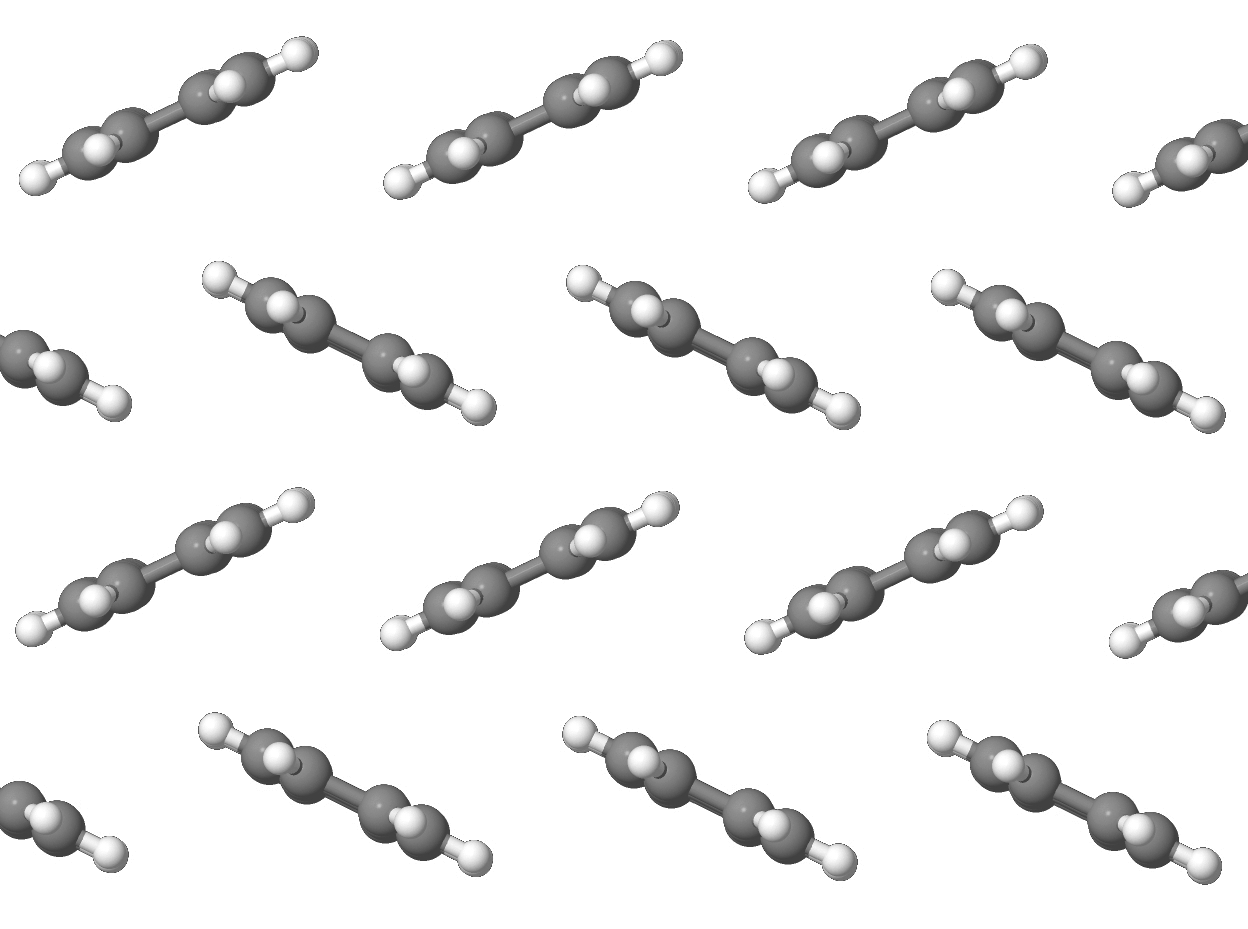
\includegraphics[width=0.4\textwidth]{../img/herringbone.png}
	\caption{An example of the \\herringbone packing \\typically found in \\Pentacene crystals}
	\label{fig:HerringbonePacking}
\end{wrapfigure}
The molecule under investigation is pentacene. This molecule is a popular organic semiconductor and the subject of much research due to its high field effect mobility \cite{Hu2005}, use in device applications \cite{Hasegawa_2009} and, more recently, the use of functionalization to alter device properties \cite{Anthony2001, Anthony2002}. The pentacene molecule consists of 5 joined benzene rings (36 atoms) and crystals typically pack with a herringbone motif as shown in figure \ref{fig:HerringbonePacking}.
\clearpage
\section{Creating Amorphous Pentacene}
In order to create the amorphous pentacene systems a melt-quench technique was used. This is a standard technique, often used to create amorphous systems in both computational and experimental  fields \cite{D’Angelo2018, PhysRevB.77.172101, BERBANO201293, KARMWAR201194, KO1996211}. The procedure followed is shown in figure \ref{fig:meltQuenchFlowChart}.
\begin{figure}[H]
	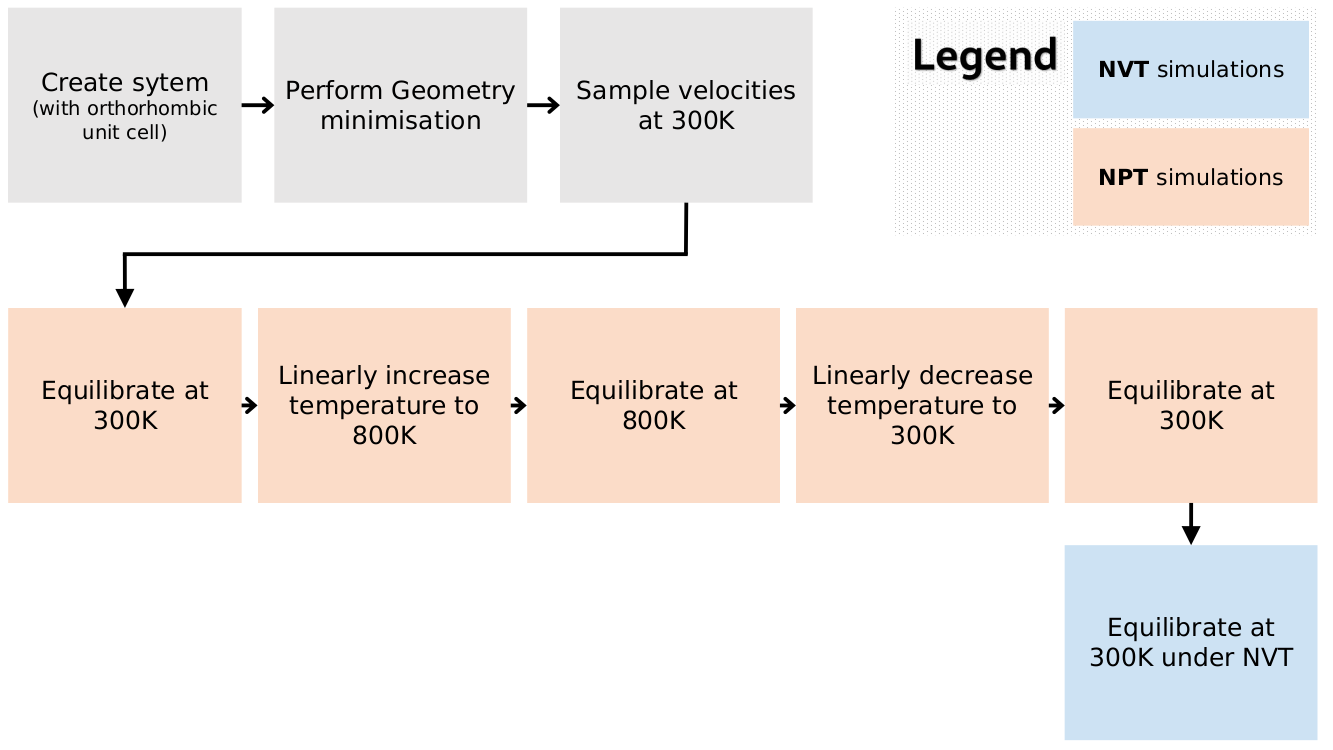
\includegraphics[width=\textwidth]{../img/FlowCharts/MeltQuench.png}
	\caption{\label{fig:meltQuenchFlowChart}The melt-quench scheme used to create amorphous pentacene systems. Blue boxes indicate steps using an NPT ensemble, orange boxes indicate use of a NVT ensemble.}
\end{figure}
\noindent In this procedure, the system was initialised with an individual pentacene molecule on a regular 3D grid using an orthorhombic unit cell. This was chosen to make analysis of the resulting structures easier than with the triclinic unit cell typically used to simulate pentacene crystals. The velocities were initially randomly sampled from a gaussian distribution and a Nose-Hoover thermostat and barostat was used to control the temperature and pressure. The Lammps molecular dynamics package was used \cite{LammpsMain, LammpsURL} and electrostatic interactions were handled with Lammps' particle-particle-particle-mesh ewald method \cite{LammpsPPPME}. RESP \cite{RESP} (restrained electrostatic potential) partial charges were parameterised using Gaussian 16 \cite{g16} with the B3-LYP\cite{B3,LYP} level of theory and a 6-311g(d) basis set. The use of partial charges was essential in the creation of the amorphous systems and neglecting them lead to unphysical face-to-face stacking of pentacene molecules. This is shown in figure \ref{fig:glob_coup}, in section \ref{sect:GlobCoup}. Finally, for inter and intra molecular interactions the general AMBER force-field \cite{GAFF} (GAFF) was applied. There isn't one predominant forcefield used in simulations of pentacene in the literature, though parameters from GAFF have been used and validated in a number of studies \cite{C0JM01577F, Yoneya2012, PentCrystallisation, MILLER201728, Wang2011, C6CP06436A, doi:10.1246/cl.180450}.
\\\\
Four different quenching times were used spanning 4 orders of magnitude: 0ns, 1ns, 10ns and 100ns. For the 0ns, 1ns and 10ns quenching simulations 3,000 molecules were simulated. In the 100ns quenched structure 3060 molecules were simulated. The initial structure for the 1ns and 10ns quenched structures were taken from a restart of the 0ns quenched simulation after the 800K equilibration step. The 0ns and 1ns quenched structure were carried out under 1 atmosphere of pressure in x, y and z. However, the 10ns quenching required a small increase to 5 atmospheres as the structure had a tendency to deform such that one of the cell vectors became either very large or very small. In the 100ns quenched structure I updated the barostat target pressure (before the phase transition) to account for similar deviations in simulation box dimensions.
\section{Structure of the quenched simulations}
A movie showing the full 100ns melt-quench simulation can be found here: \href{https://youtu.be/6IQcYErQHVs}{https://youtu.be/6IQcYErQHVs}. Still images of the final snapshot of each different quenching time are shown in figure \ref{fig:final_snapshots}.
\subsection{Final Structure Snapshots}
\noindent We can see qualitatively that as we increase the quenching time from a) $\rightarrow$ d) the structure starts to look more ordered and crystal layers are starting to be formed. Looking longer at the structure we see that lower quench times tend to form small crystal clusters. In the 0ns quenched structure these clusters tend to be just $\sim$7-10 molecules in size. As we increase the quenching time to 1ns we see 1D channels of crystalline pentacene start to form throughout the structure, though the structure is still relatively disordered due to these channels being randomly oriented with respect to one another. As we increase the quenching time these crystal fragments become larger until in the 100ns quenched structure the whole system is comprised of just 2 crystals. The reason for this is, as the rate of cooling is decreased, the rate of crystal seeding is also decreased. At longer quenching times, more spent is spent at a temperature where it is unlikely for crystal to start to form --so fewer form. Those that do form can therefore propagate through the full system before being impeded by others. This can be seen in the animation of the \href{https://youtu.be/6IQcYErQHVs}{100ns melt quench simulation} linked above. The reverse is true for the shorter quenching times. In these systems, we quickly pass into a state that's energetically favourable for many crystals to start to form. These all propagate out at random orientations with respect to each other and block each other's growth.

\begin{figure}[ht]
	\includegraphics[width=\textwidth]{../img/DifferentQuenchTimes/AllTimes.png}
	\caption{\label{fig:final_snapshots}The final snapshot of each quenching simulation visualised in VMD \cite{VMD} and rendered with Tachyon \cite{Tachyon}. Snapshots are ordered by quenching time i.e. a) is the 0ns quench, b) is the 1ns quench and so on.}
\end{figure}
\subsection{Molecular Packing}
\noindent We can isolate clusters in each of the different structures shown in figure \ref{fig:final_snapshots} to reveal the molecular packing within. In figure \ref{fig:Layer11} a DBSCAN\cite{DBSCAN}-like algorithm has been applied to the final structure from the 100ns quench to cluster molecules based on the density of centers of mass of molecules. These clusters have then been highlighted by different colours. The top-most green cluster has been rotated such that, on the left, we are viewing it at an angle perpendicular to the plane of molecules, as shown by the cartoon eye. Comparing this plane to the crystal plane to the right, we can see a striking similarity in the packing motif. The herringbone packing has formed and (as can be seen in figure \ref{fig:ang_dist} in section \ref{sect:ang_dist}) the herringbone intersection angle is remarkably similar to that of the crystal plane. This serves as a confirmation of the choice of force-field and the parameterisation of the partial charges.
\begin{figure}[ht]
	\includegraphics[width=\textwidth]{../img/DifferentQuenchTimes/100ns/Layer11_Demonstration.png}
	\caption{\label{fig:Layer11}The 100ns quenched structure with different clusters shown with different colours. A bird's eye view of the green cluster has been shown on the left to demonstrate the herringbone packing within each cluster/layer. The far-right image labelled `Crystal' is a snapshot of a crystal plane after a short MD equilibration.}
\end{figure}
\begin{wrapfigure}[11]{r}{0.45\textwidth}
	\centering
	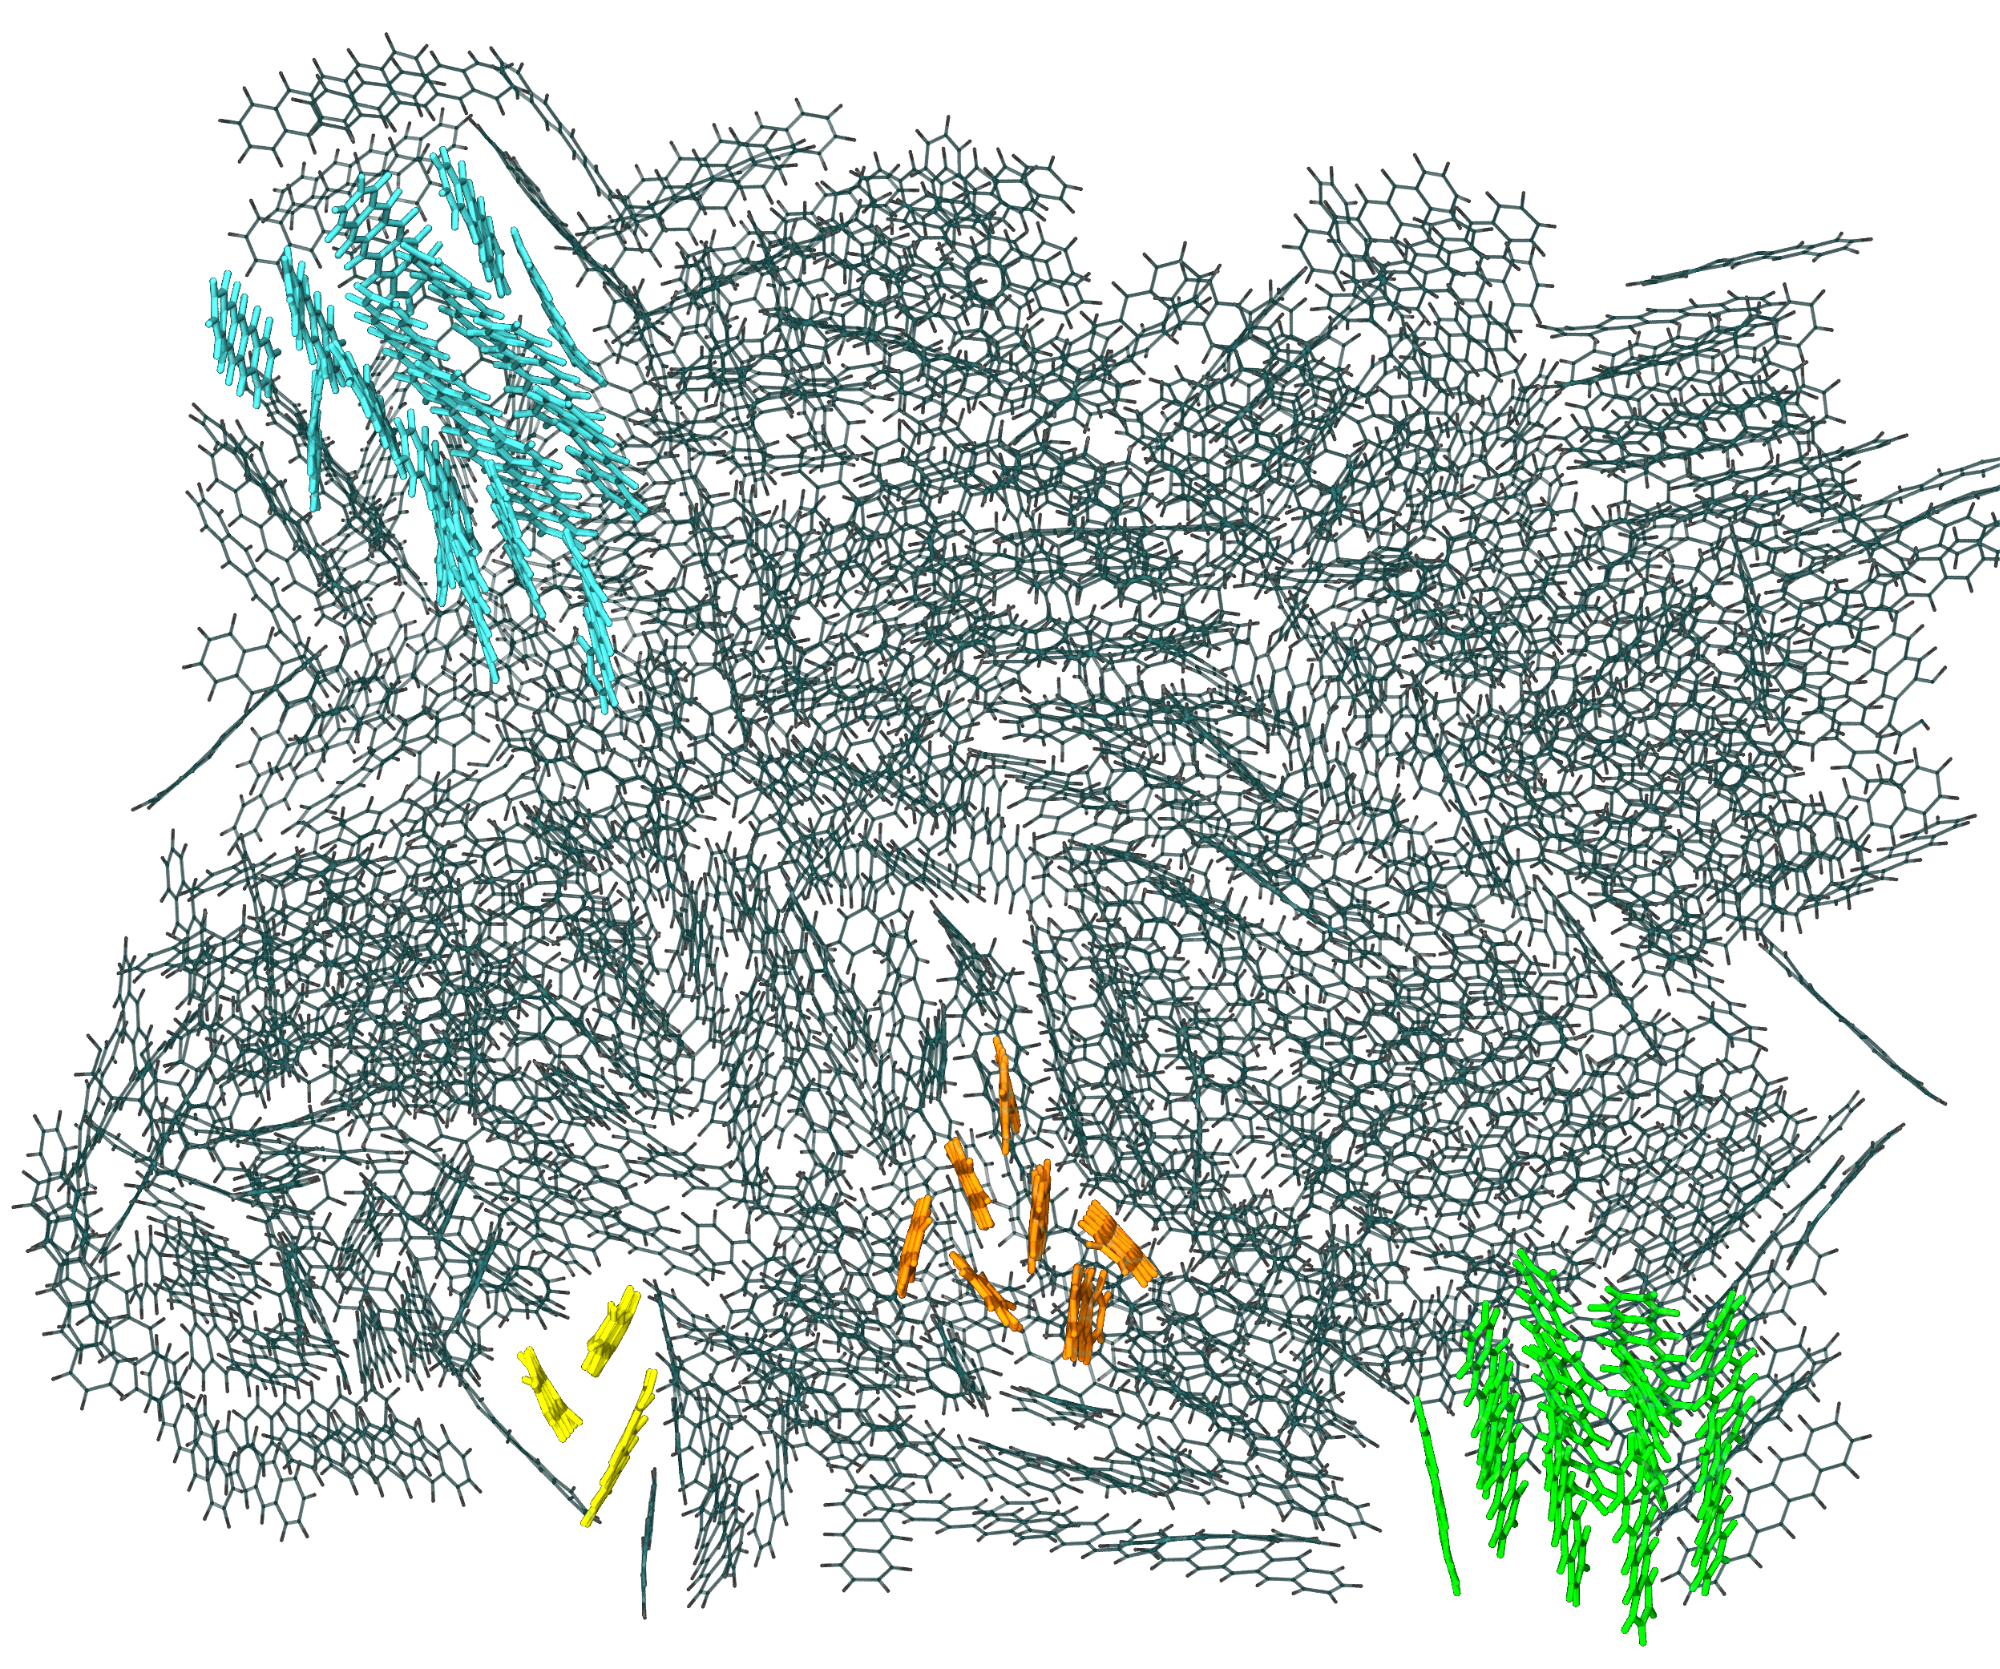
\includegraphics[width=0.45\textwidth]{../img/DifferentQuenchTimes/0ns/Slice6_4Clusters.png}
	\caption{\label{fig:ClustInst}A slice from the 0ns quenched structure with 2 selected clusters displaying herringbone-like packing.}
\end{wrapfigure}
Although this herringbone packing pattern is most obvious in the 100ns quenched structure, it can also be seen in the other structures. At the other extreme in the 0ns quenched structure we see tiny clusters ($<$10 mol) of pentacene crystals forming. This is shown in figure \ref{fig:ClustInst}. At this quenching time (0-50 ps) it was energetically favourable for many regions of the structure to start to crystallise at once. This resulted in a high density of crystal fragments growing into each other and stopping when a neighbouring crystal fragment was encountered. In figure \ref{fig:ClustInst}, 2 such clusters are shown in blue and green. In both clusters the packing motif has become very herringbone-like. However, due to their small size they are more affected by the surrounding environment which warps the structure slightly. 
\\\\
\noindent To quantify the change in the structure for the differently quenched structures 3 macroscopic properties have been plotted: the mass density, the angular distribution and the radial distribution function. These are discussed in the following sections.
\subsection{Mass Density}
\begin{figure}[ht]
	\centering
	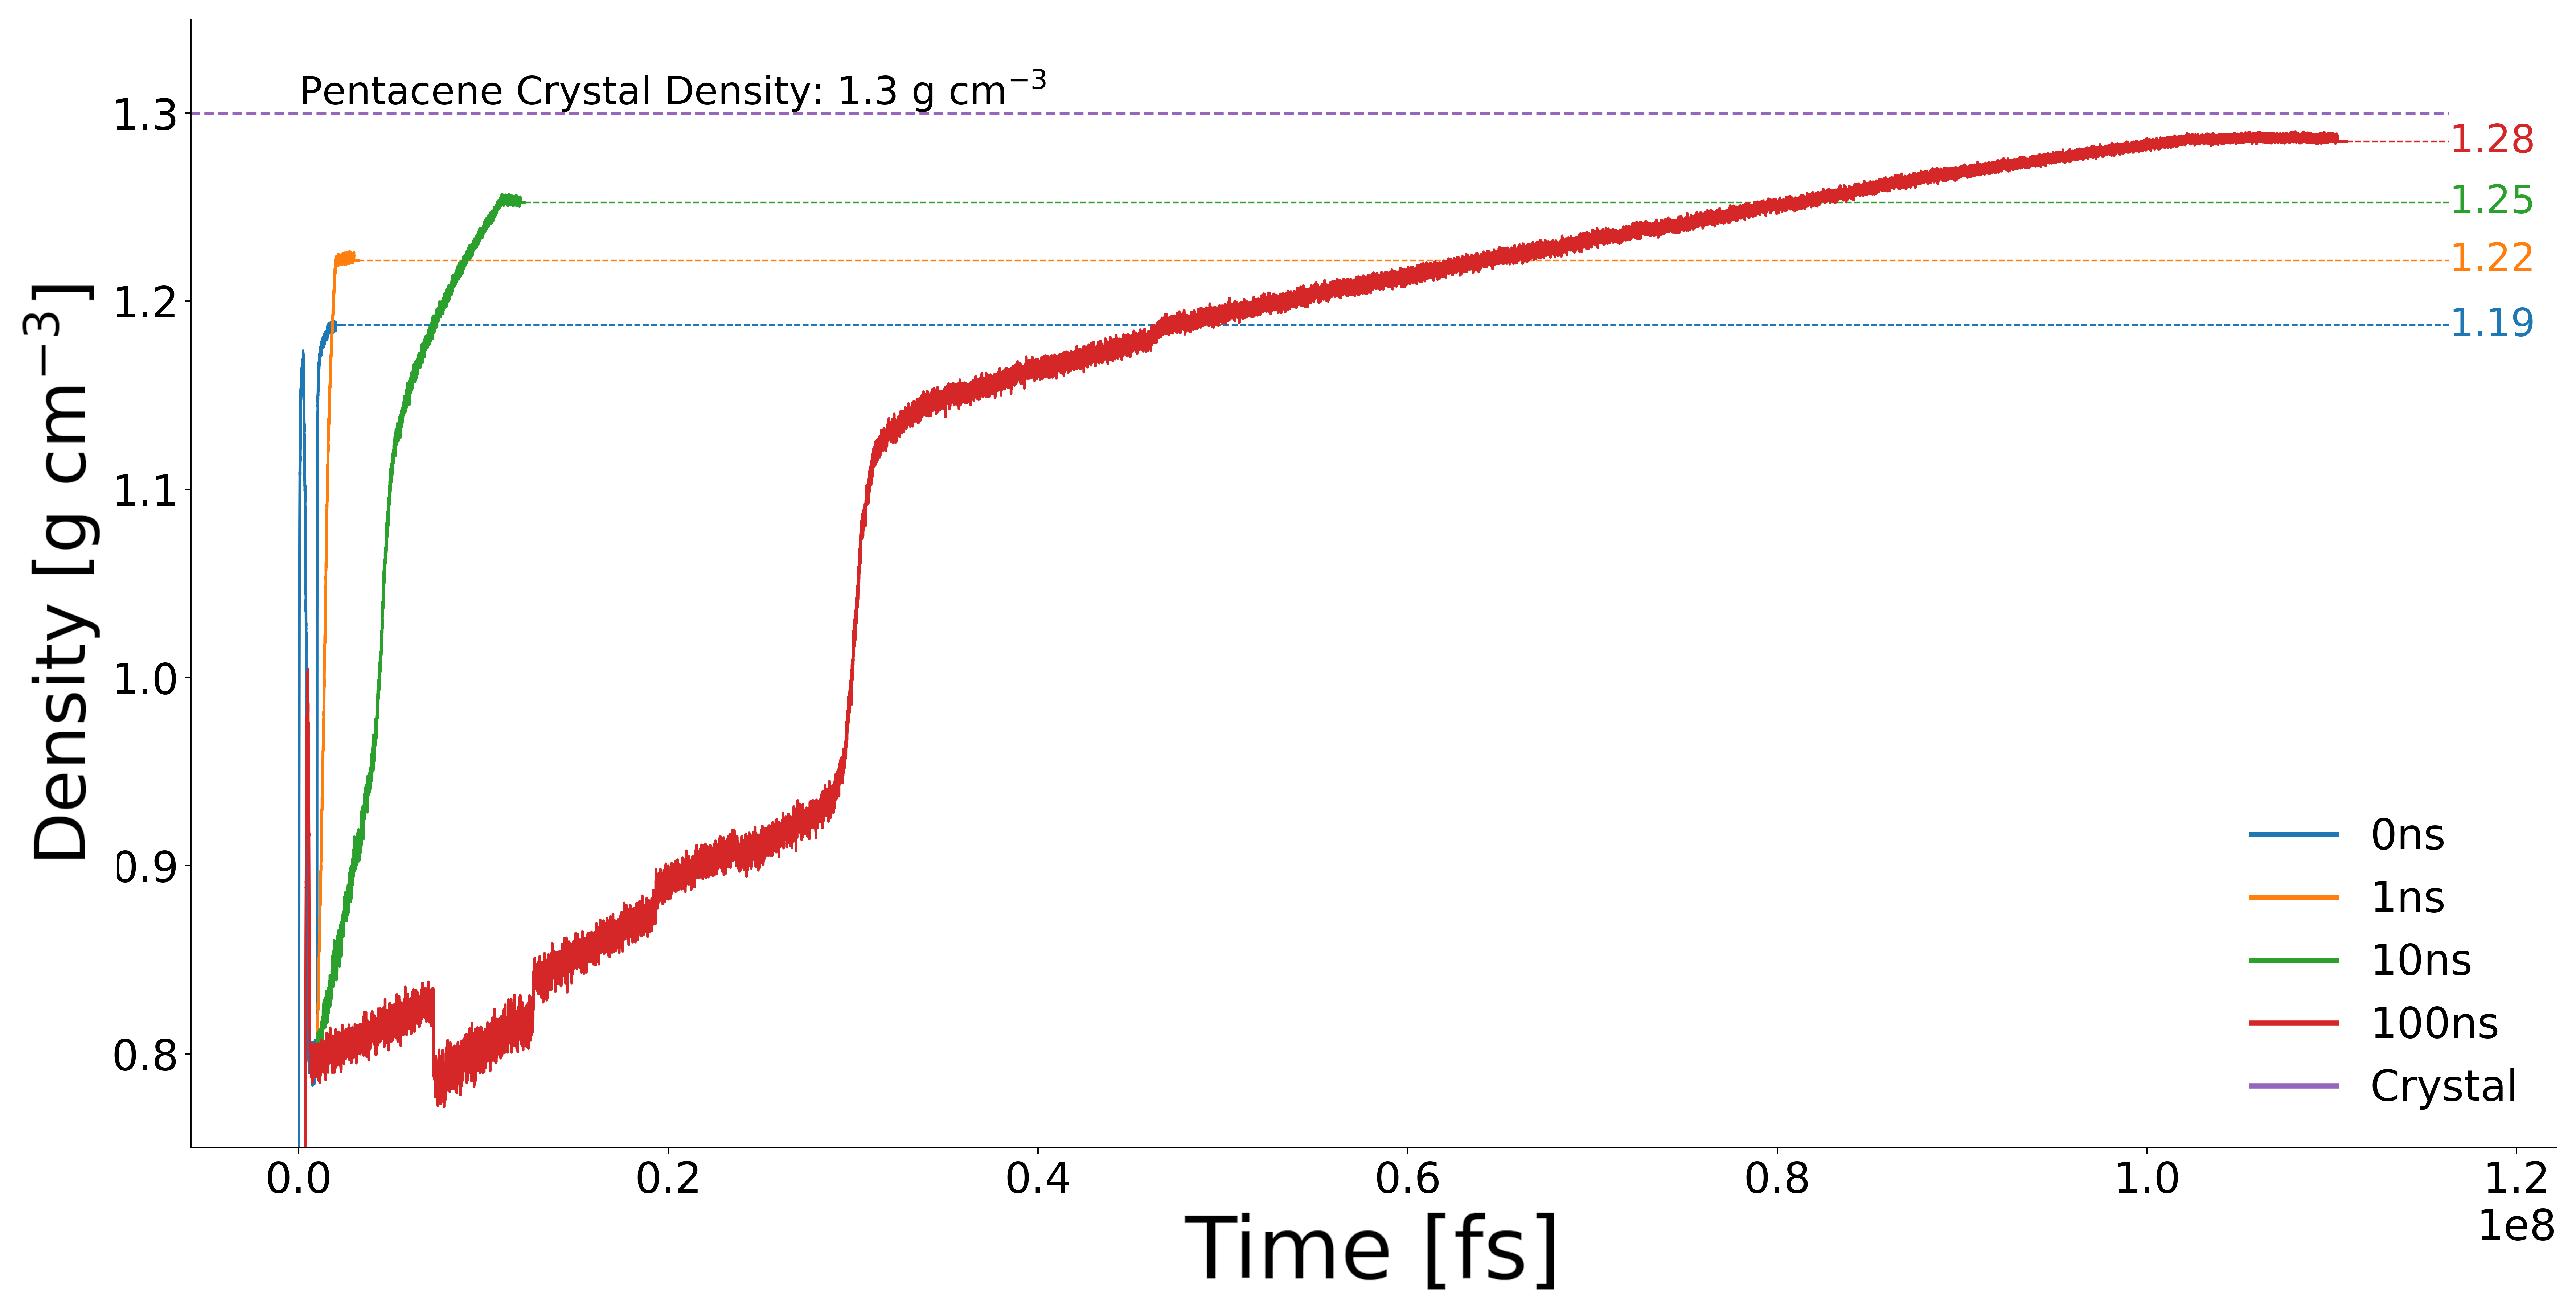
\includegraphics[width=0.9\textwidth]{../img/DifferentQuenchTimes/Density.png}
	\caption{\label{fig:QuenchDensity}A time series of the density of the quenched structures. The black line shows the experimental mass density of crystal pentacene.}
\end{figure}
\noindent The mass density of the 4 different quenching simulations can be seen in figure \ref{fig:QuenchDensity}. This was calculated by dividing the total mass of the atoms in the system by the volume (product of cell vectors) of the simulation box. The first thing to notice in this graph is as we increase the quenching time we increase the density of the final sample. This is due to the molecules packing more efficiently in the crystal than in an amorphous structure. We also see very clearly in the plots the sudden increase in density associated with the phase transition from liquid to solid Pentacene. In the 1ns quench structure (quenched with the barostat set to 1 atmosphere) this occurs around Pentacene's experimental melting of 530.15K \cite{PentaceneMeltingPoint} providing confirmation of the choice of force-field. The 0ns, 1ns and 10ns runs were performed in a single 24 hour run. The 100ns quench was performed using many restarts, the discontinuities in the density for the 100ns structure come from these restarts. These do not affect the final structure as these only occur while the system is in the liquid state.

\subsection{Angular Distribution}
\label{sect:ang_dist}
\begin{figure}[ht]
	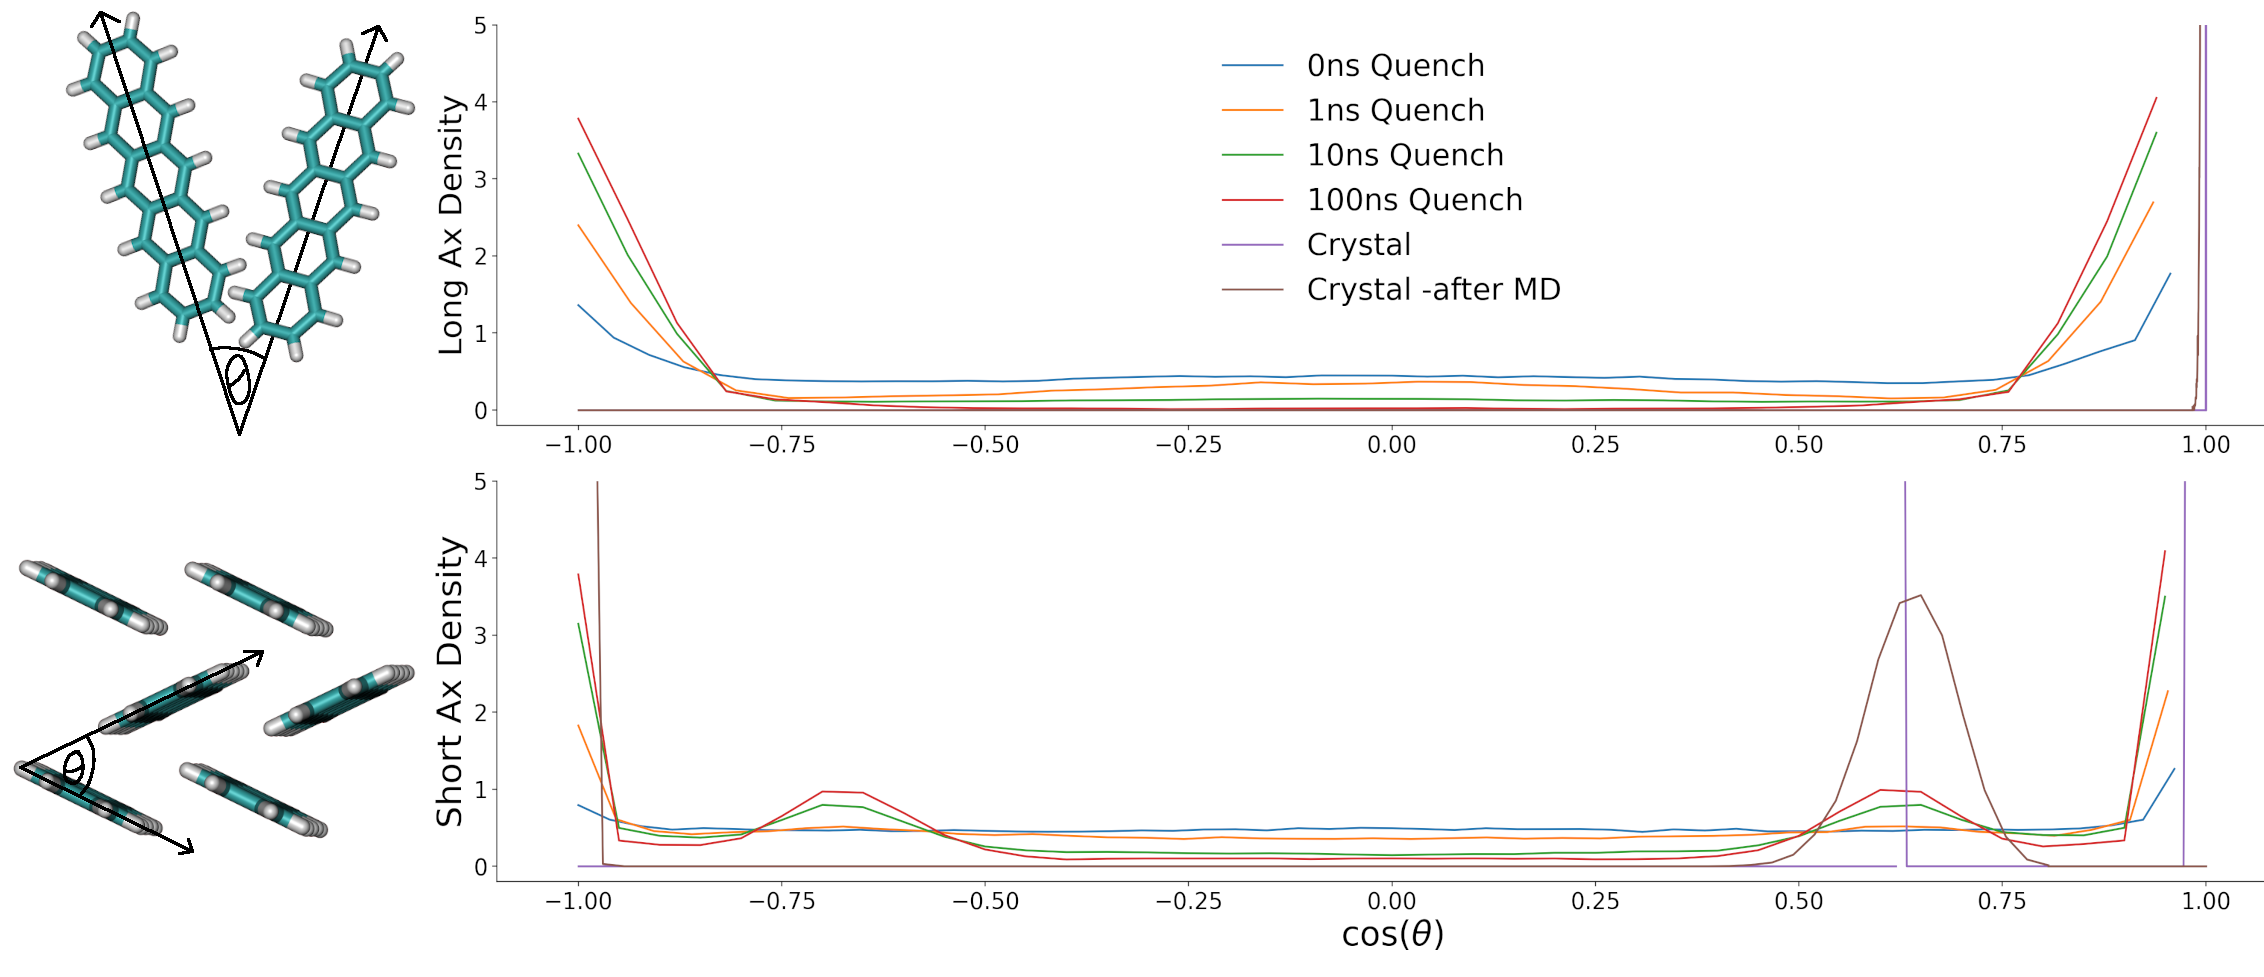
\includegraphics[width=\textwidth]{../img/DifferentQuenchTimes/AngularDist.png}
	\caption{\label{fig:ang_dist}
\noindent The angular distribution for the 4 different quench times is shown above. The brown and purple lines are from a perfect crystal before and after a short MD run. The others are after the various melt-quench simulations. On the right is a schematic showing which angles are referenced in each plot.}
\end{figure}
\noindent The angular distribution shows the distribution angles each molecule makes with the other molecules in the system. In figure \ref{fig:ang_dist} it was calculated by calculating the angle of an axis of each molecule with its nearest neighbours (a 20$\angstrom$ center of mass cutoff was used). This data was then grouped into a histogram which is plotted.
In figure \ref{fig:ang_dist} we can see as the quenching time increases we start to notice an ever more prominent peak appear at either extreme of the x axis. This is because the molecules are aligning parallel with one another. The symmetry of the plot is an artefact of the melt stage of the simulation were each molecule was free to rotate randomly.
\\\\
If we now look at the short axis plot we can see that, again, as the quench time increases we start to see a more ordered structure start to form. This time the herringbone intersection angle between molecules (54.3$^{o}$ \cite{PentaceneAngle}) within the herringbone structure is retrieved. This is a result of using partial charges in the simulation -running the same simulations without partial charges results in an unrealistic face-to-face stacking. The brown and purple line show the same calculation run on a crystal of pentacene before and after MD. The purple line comes from an analysis of a repeated unit cell, hence we get 2 delta functions: one at 54.3$^{o}$ and one at 0$^{o}$. This structure was then equilibrated with electrostatics for 50ps and we start to see a broadening of the herringbone intersection angle and to a lesser extent (on the left side) a broadening of the angle between parallel pairs.
\subsection{Radial Distribution Function}
\begin{figure}[H]
	\centering
	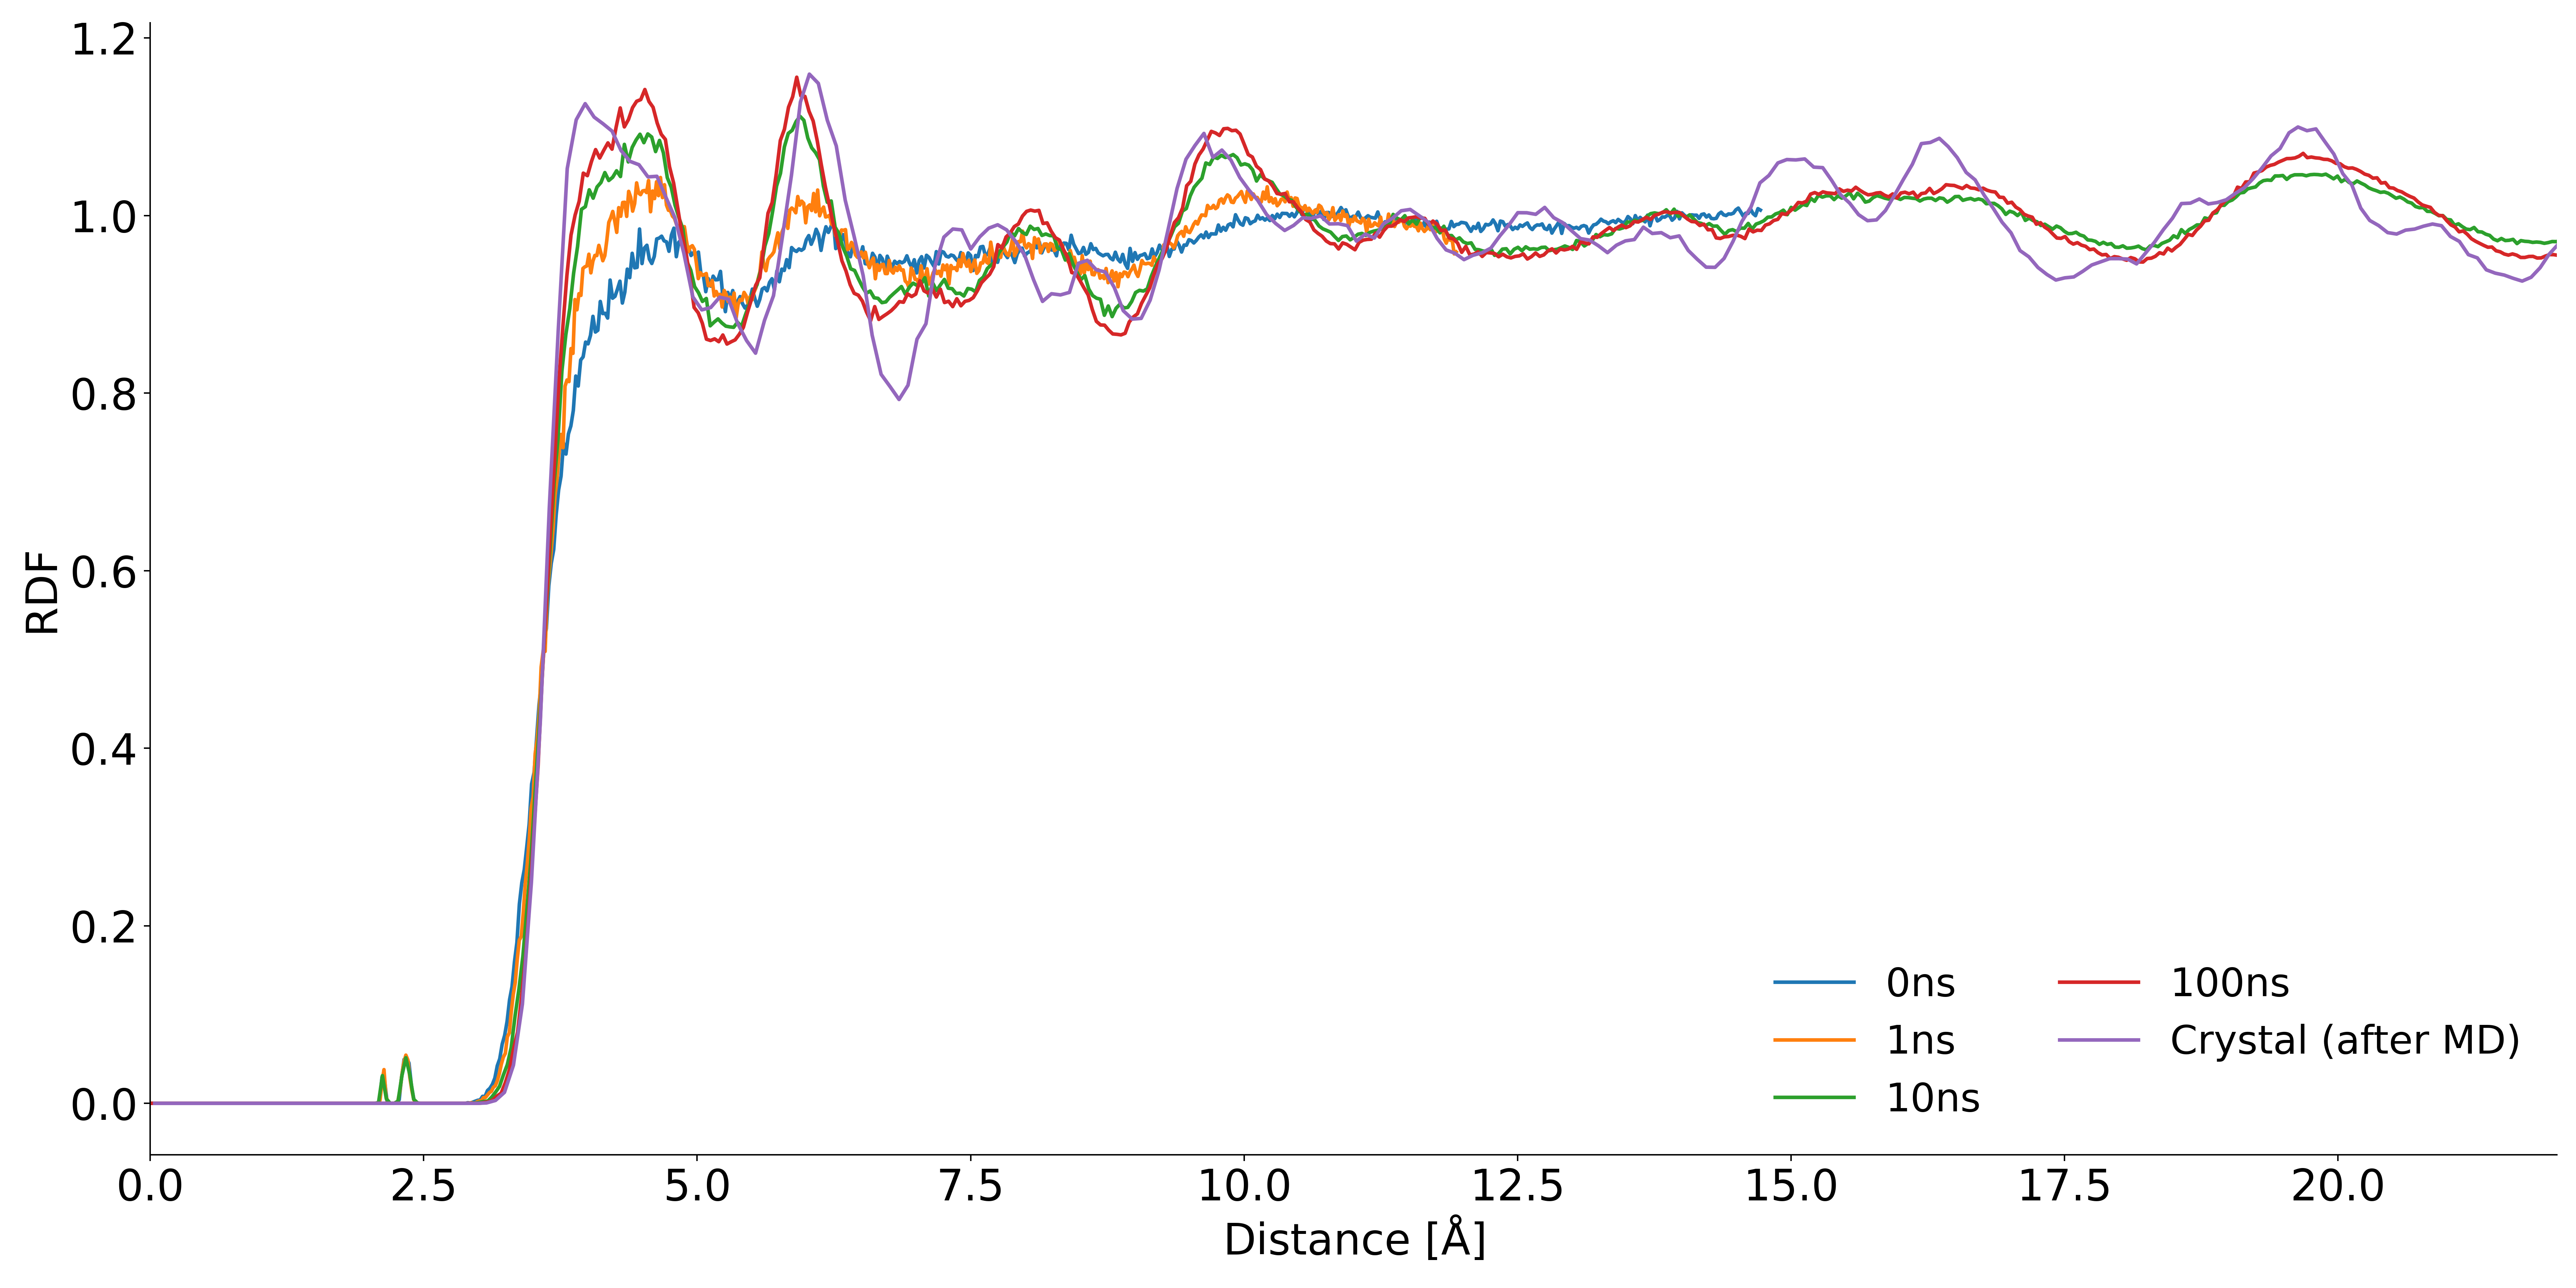
\includegraphics[width=\textwidth]{../img/DifferentQuenchTimes/RDF.png}
	\caption{\label{fig:RDF}The carbon-carbon radial distribution function for 4 different quenching times and a crystal before and after 50ps of MD. The quenches (0, 1, 10 and 100ns) are shown in blue, orange, green and red respectively. The crystal data are shown in purple and brown.}
\end{figure}
\noindent The radial distribution function (RDF) describes the change of density from each particle in the system and is normalised to the bulk density (i.e. $\frac{N}{V}$). This was calculated by counting the number of atoms within a spherical shell from each atom and then dividing by the volume between these spheres. This local density was then normalised to the bulk crystal density. In systems with atoms regularly placed throughout the system we would expect to see sharp peaks in the RDF as there would be many gaps with no atoms. Conversely, with a totally amorphous system we would expect to see (once we reach a few times the Van der Waals radius from each atom) a flat line at 1 as local density should be very similar to the global density. This pattern is what we observe in figure \ref{fig:RDF}. The sharp peaks of the purple line show the RDF of a perfect crystal (repeated unit cell) confirming we have a highly ordered system. On the other extreme, the blue line shows very weak ordering of the atoms' positions with any ordering vanishing after $\sim$12.5$\angstrom$ from each atom. This is due to the 0ns structure comprising primarily of small crystal fragments giving rise to a small amount of very local order but over longer distances this order vanishes. Again, as the quench time increases, the ordering increases resulting in larger peaks that more closely match the RDF of the crystal after a short MD equilibration.

%\subsection{Orientational Order Parameter}
%\begin{figure}[ht]
%	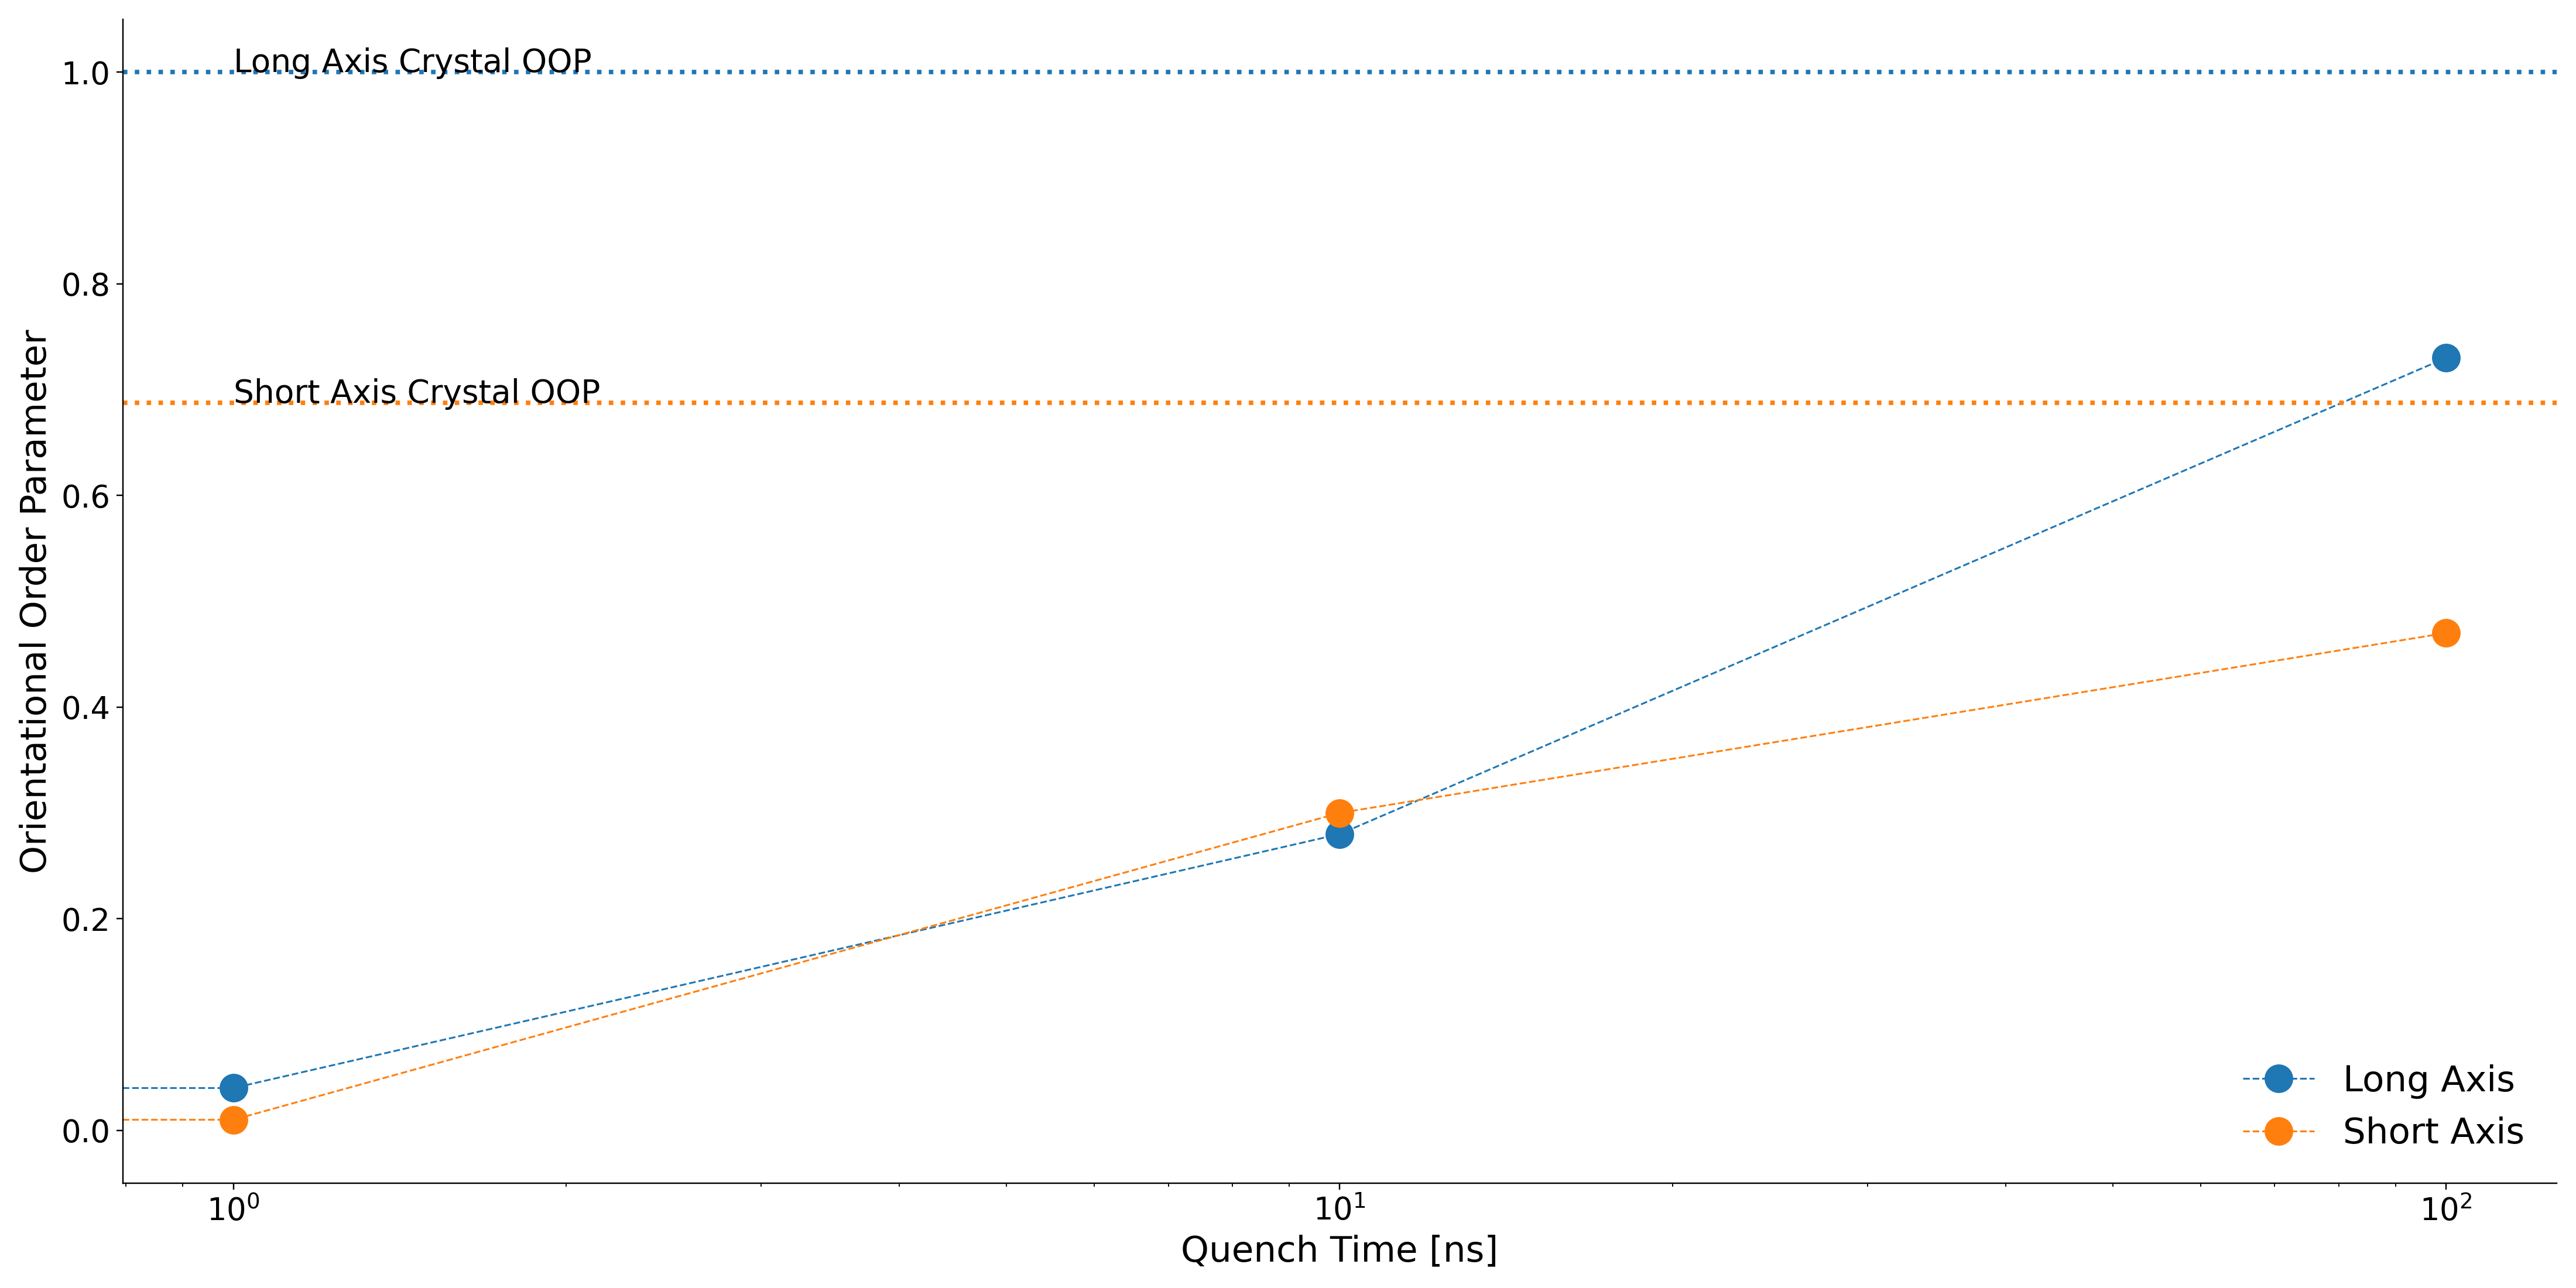
\includegraphics[width=\textwidth]{../img/DifferentQuenchTimes/TimevsOOP.png}
%	\caption{\label{fig:OOP}The change in the orientational order parameter (OOP) with respect to the quenching time. The blue data represents the values for the long axis and the orange data represents the short axis values. The horizontal lines show the theoretical value for a perfect crystal.}
%\end{figure}
%\noindent The orientational order parameter gives a single number describing how aligned the molecules within a system are. Values lie on a scale from -0.5 to 1, where 1 denotes all molecules are aligned, 0 denotes a random alignment of molecules and -0.5 denotes an anti-alignment with respect to the reference vector. The formula for the orientational order parameter is given below in equation \eqref{eq:OOP}.
%\begin{equation}
%	S = \frac{3}{2} \ \frac{1}{N_{mol}}\sum_{i}^{N_{mol}} \left[\frac{\mathbf{v}_{i} \cdot \mathbf{v}_{ref}}{|\mathbf{v}_{i}| |\mathbf{v}_{ref}|} \right]^{2}  - \frac{1}{2}
%	\label{eq:OOP}
%\end{equation}
%Where $\mathbf{v}_{i}$ is the vector describing the long or short axis of molecule i. The reference vector $\mathbf{v}_{ref}$ was defined as the average over $\mathbf{v}_{i}$ i.e: $\mathbf{v}_{ref} = \left\langle \mathbf{v}_{i} \right\rangle_{i}$. $N_{mol}$ is the number of molecules and i indicates a molecule index.
%\\\\
%In figure \ref{fig:OOP} we can see the change in the orientational order parameter with quenching time and, as seen in the previous sections, as we increase the quenching time we increase (orientational) order in the system. This isn't surprising as this quantity is very similar to the angular distribution.

\subsection{Crystallinity}
In order to quantify the level of order within the system, an estimator of crystallinity based on the final mass density of the superstructure was used. The formula for this is presented below in equation \eqref{eq:crystallinity}
\begin{equation}
  C = 100 \left(\frac{\rho_{sample} - \rho_{amorphous}}{\rho_{crystal} - \rho_{amorphous}}\right)
  \label{eq:crystallinity}
\end{equation}
This estimator simply linearly interpolates between the minimum (amorphous) density, $\rho_{amorphous}$, and the maximum (crystal) density, $\rho_{crystal}$. The relationship between the quenching time and this definition of crystallinity is shown in figure \ref{fig:crystallinity}. Note in this figure, the quench time 0ns is missing. This is because the system didn't equilibrate instantly and it took approximately 100ps for the density to converge. It can be seen in this figure, that surprisingly, the crystallinity (final density) increases almost exactly logarithmically with respect to quench time. The black dashed line shows a line of best fit using the equation $C = m log_{10}(t) + C_{0}$ as a guide for the eye. This crystallinity parameter will be used when looking at the electronic transport properties (hole mobility and IPR) in the following section, in order to compare the electronic transport properties to a physically meaningful property.
\begin{figure}[htp]
  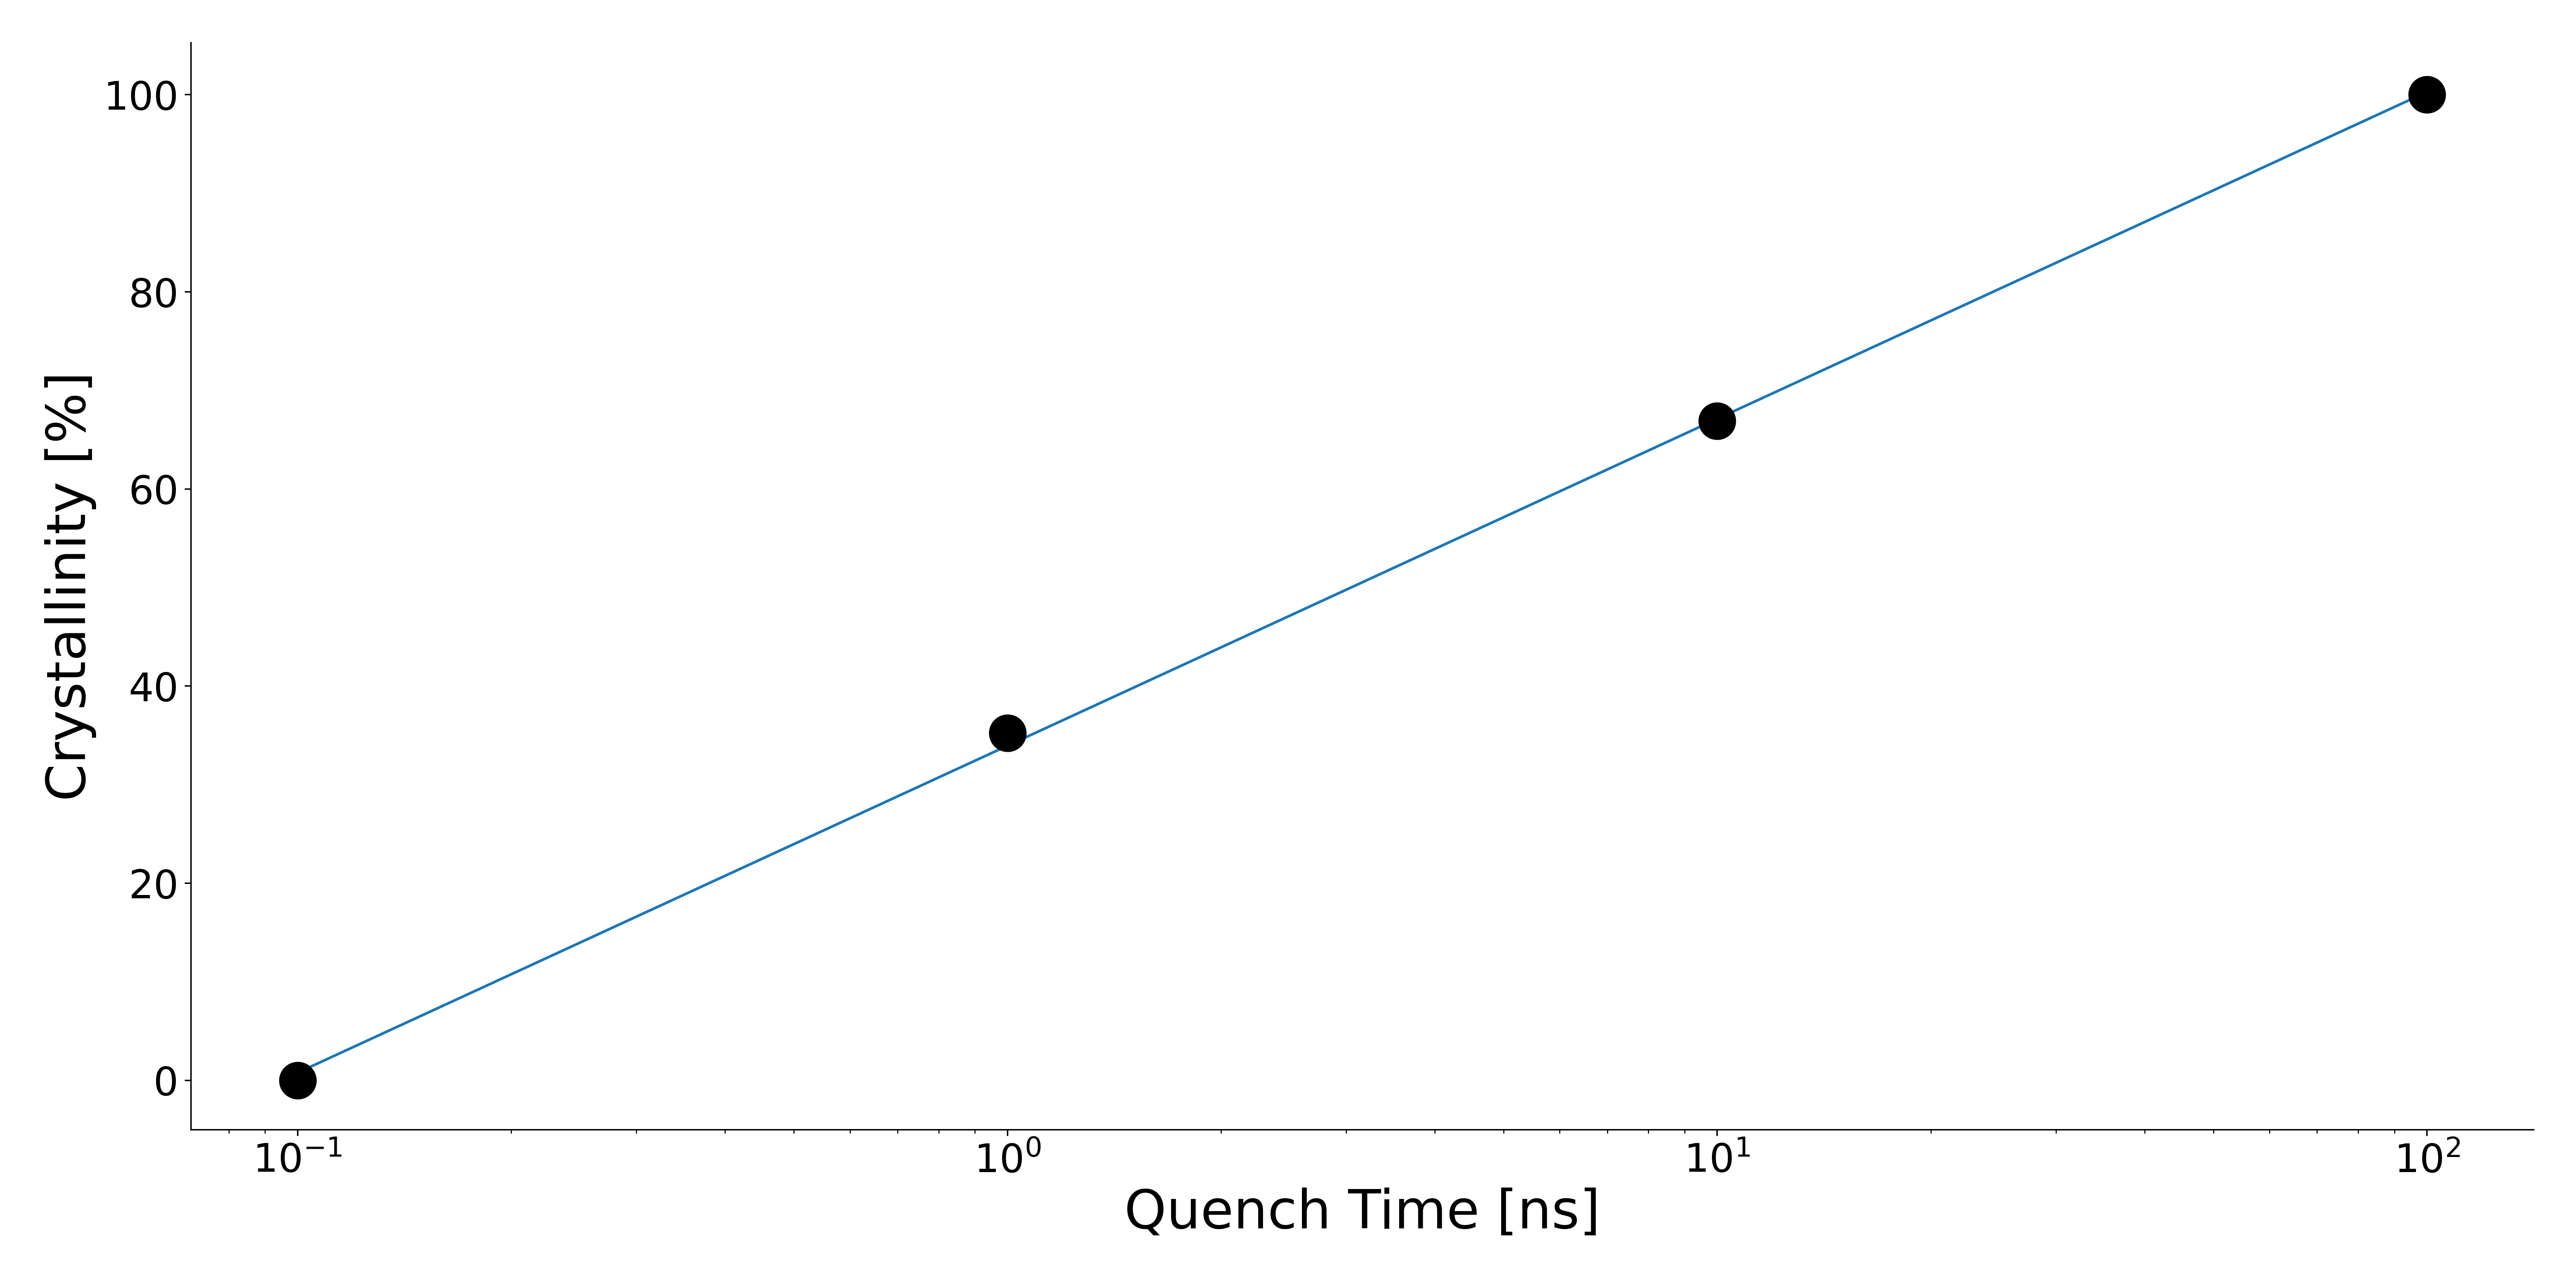
\includegraphics[width=\textwidth]{../img/DifferentQuenchTimes/QuenchTvsCrystallinity.png}
  \caption{\label{fig:crystallinity}The quench time vs crystallinity given by equation \ref{eq:crystallinity}. Black circles show raw data and the dashed black line is a line of best fit using the equation $C = m log_{10}(t) + C_{0}$.}
\end{figure}

